%\input{preamble.txt}
%
%\begin{document}
\section{SOLID Design}

\begin{itemize}
	\item What is SOLID?
	\begin{itemize}
		\item \textbf{S}ingle Responsibility Principle
		\item \textbf{O}pen/Closed Principle
		\item \textbf{L}iskov Substitution Principle
		\item \textbf{I}nterface Segregation Principle
		\item \textbf{D}ependency Inversion Principle
	\end{itemize}

	\item Single Responsibility Principle (SRP)\\
	\textbf{\emph{A class should have only one reason to change}}
	\begin{itemize}
		\item If you can think of more than one motive for changing a class, then that class has more than one responsibility
		\item If a class has more than one responsibility, then the responsibilities become coupled
		\item Violating the SRP\\
		\begin{center}
			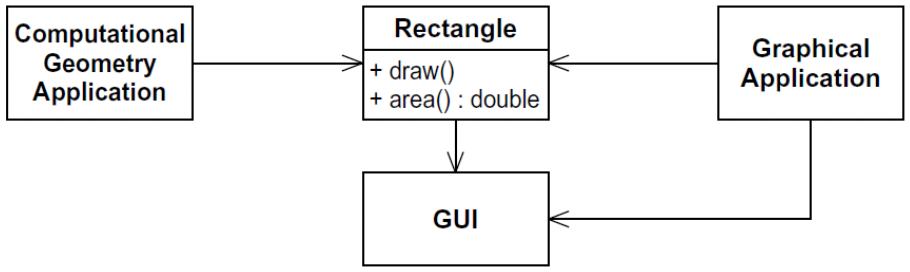
\includegraphics[width=0.6\linewidth]{SRPViolation}
		\end{center}
		\item Conforming to the SRP
		\begin{center}
			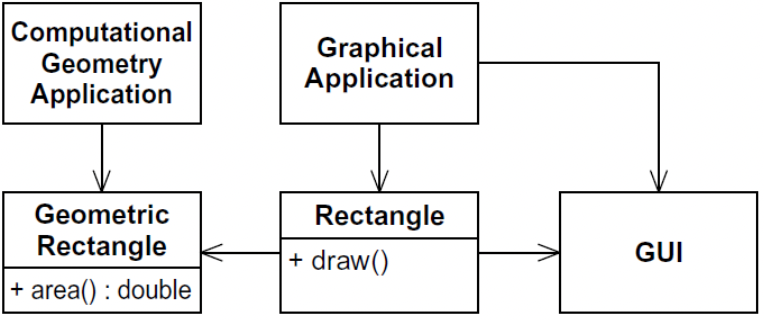
\includegraphics[width=0.5\linewidth]{SRPConform}
		\end{center}
	\end{itemize}

	\item The Open/Closed Principle (OCP)\\
	\textbf{\emph{Software entities (classes, modules, functions, etc.) should be open for extension, but closed for modification.}}
	\begin{itemize}
		\item When a single change to a program results in a cascade of changes to dependent modules, the design smells of rigidity.
		\begin{itemize}
			\item If the Open/Closed principle is applied well, then further changes of that kind are achieved by adding new code, not by changing old code that already works.
		\end{itemize}
		\item In Java, it is possible to create abstractions that are fixed and yet represent an unbounded group of possible behaviors
		\begin{itemize}
			\item The abstractions are abstract base classes, and the unbounded group of possible behaviors is represented by all the possible derivative classes.
		\end{itemize}
		\item Violating the OCP
		\vspace{\itemsep}
		\vspace{\parsep}
		\begin{itemize}
			\begin{minipage}{0.5\textwidth}
				\item Both classes are concrete
				\item The \textbf{Client} uses the \textbf{Server} class
			\end{minipage}
			\begin{minipage}{0.5\textwidth}
%				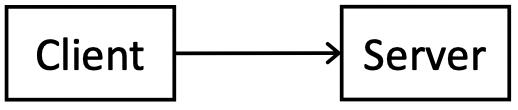
\includegraphics[width=1.5in]{OCPViolate}
%				\begin{figure}
%					\centering
					\begin{tikzpicture}

						\node[rectangle,draw] (client) at (0,0) {\Verb|Client|};

						\node[rectangle,draw] (server) [right=of client,] {\Verb|Server|};

						\draw[-Straight Barb] (client) -- (server);

					\end{tikzpicture}
%				\end{figure}
			\end{minipage}
		\end{itemize}

		\begin{minipage}{0.5\textwidth}
			\item Conforming to the OCP\\
		\end{minipage}
		\begin{minipage}{0.5\textwidth}
%			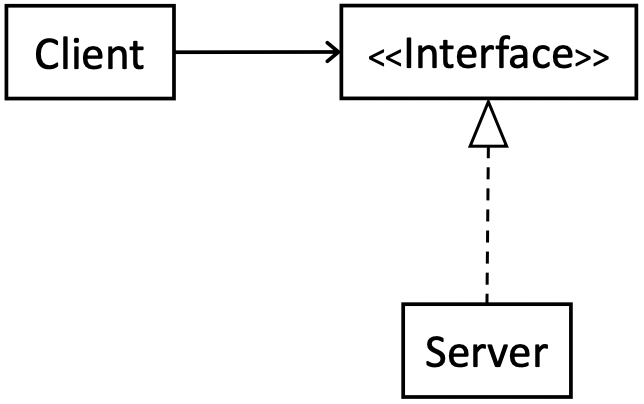
\includegraphics[width=0.4\textwidth]{OCPConform}
			\begin{tikzpicture}

				\node[rectangle,draw] (client) at (0,0) {\Verb|Client|};

				\node[rectangle,draw] (interface) [right=2cm] {\Verb|<<Interface>>|};

				\node[rectangle,draw] (server) [below=1cm of interface,] {\Verb|Server|};

				\draw[-Straight Barb] (client.east) -- (interface.west);

				\draw[dash pattern=on 2pt off 1pt, -{Triangle[open]}] (server.north) -- (interface.south);

			\end{tikzpicture}
		\end{minipage}
	\end{itemize}

	\item The Liskov Substitution Principle (LSP)\\
	\textbf{\emph{Subtypes must be substitutable for their base types.}}
	\begin{itemize}
		\item Formally: Let $ \Phi(x) $ be a property provable about objects $ x $ of type $ T $. Then $ \Phi(y) $ should be true for objects $ y $ of type $ S $ where $ S $ is a subtype of $ T $.
		\item Counter-example: ``If it looks like a duck, quacks like a duck, but needs batteries – you probably have the wrong abstraction"
		\item Violating the LSP\\
		Issues:\\
		\begin{minipage}{0.6\textwidth}
			\begin{itemize}
				\item Inheriting \textbf{height} and \textbf{width}
				\item Overriding \textbf{setHeight} and \textbf{setWidth}
				\item Conflicting assumptions. For example:
				\begin{Verbatim}
	void testRectangleArea(Rectangle r){
		r.setWidth(5);
		r.setHeight(4);
		assertEquals(r.computeArea(), 20);
	}
				\end{Verbatim}
			\end{itemize}
		\end{minipage}
		\begin{minipage}{0.3\textwidth}
%			\hspace*{2cm}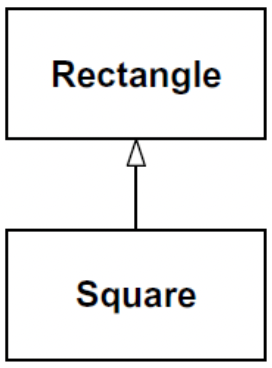
\includegraphics[width=1in]{LSPExample}
			\begin{tikzpicture}
				\node[type] (Square) {\Verb|Square|};
				\node[type] (Rectangle) [above=of Square] {\Verb|Rectangle|};

				\draw[thick, -{Triangle[open, length=2.5mm, scale=1.3]}] (Square) -- (Rectangle);
			\end{tikzpicture}
		\end{minipage}

		\item Implication: A model, viewed in isolation, cannot be meaningfully validated.
		\begin{itemize}
			\item The validity of a model can only be expressed in terms of its clients.
			\item One must view the design in terms of the reasonable assumptions made by
			the users of that design.
		\end{itemize}
	\end{itemize}

	\item The Interface Segregation Principle (ISP)\\
	\textbf{\emph{Clients should not be forced to depend on methods that they do not use.}}
	\begin{itemize}
		\item This principle deals with classes whose interfaces are not cohesive. That is, the interfaces of the class can be broken up into groups of methods where each group serves a different set of clients.
		\item When clients are forced to depend on methods that they don’t use, then those clients are subject to changes to those methods.\\
		\begin{minipage}[t]{0.4\textwidth}
			\item Violating the ISP\\
%			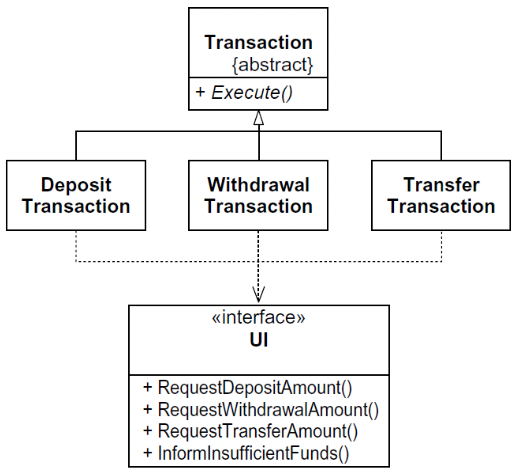
\includegraphics[width=2.5in]{ISPViolation}

			\resizebox{2.5in}{!}{	\begin{tikzpicture}
					\node[rectangle, align=center, draw] (withdrawal) {\Verb|Withdrawal| \\ \Verb|Transaction|};
					\node[rectangle, align=center, draw] (deposit) [right=of withdrawal]{\Verb|Deposit| \\ \Verb|Transaction|};
					\node[rectangle, align=center, draw] (transfer) [left=of withdrawal] {\Verb|Transfer| \\ \Verb|Transaction|};

					\node[rectangle, align=left, draw, minimum width=1in] (withdrawaltype) [above=of withdrawal] {\textit{+ Execute()}};
					\node[rectangle, align=right, draw, minimum width=1in] (transaction) [above=0pt of withdrawaltype] {\Verb|Transaction| \\ \{abstract\}};
					\coordinate (ghost) [above= 10pt of withdrawal] {};

					\draw (deposit.north) |- ([yshift=25pt]ghost) -| (transfer.north);
					\draw[-{Triangle[open, length=2.5mm, scale=1.3]}] (withdrawal) -- (withdrawaltype);

					\node[type, text width=2.2in] (ui) [below=of withdrawal] {\textbf{$ \langle\langle $Interface$ \rangle\rangle $} \\ \Verb|UI|};
					\node[method, text width=2.2in] () [below=0pt of ui] {+ RequestDepositAmount() \\ + RequestWithdrawalAmount() \\ + RequestTransferAmount() \\ + InformInsufficientFunds()};
					\coordinate (ghost2) [below= 10pt of withdrawal] {};

					\draw[densely dotted] (deposit.south) |- ([yshift=-25pt]ghost2) -| (transfer.south);
					\draw[densely dotted, -{Straight Barb[length=2mm, width=2mm]}, thick] (withdrawal) -- (ui);
				\end{tikzpicture} }
		\end{minipage}
		\begin{minipage}[t]{0.6\textwidth}
			\item Conforming to the ISP\\
%			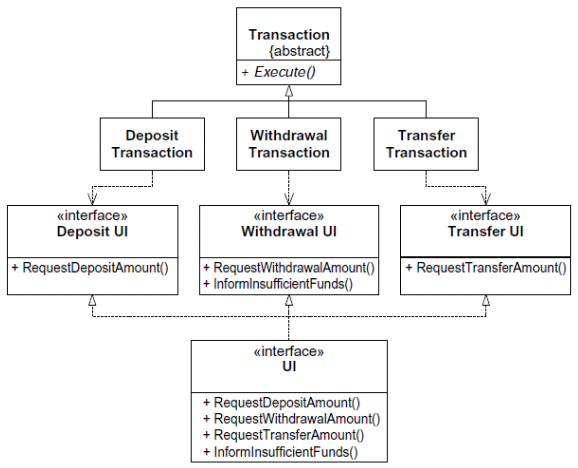
\includegraphics[width=3.5in]{ISPObey}

			\resizebox{4in}{!}{
				\begin{tikzpicture}
					\node[rectangle, align=center, draw] (withdrawal) {\Verb|Withdrawal| \\ \Verb|Transaction|};
					\node[rectangle, align=center, draw] (deposit) [left=of withdrawal]{\Verb|Deposit| \\ \Verb|Transaction|};
					\node[rectangle, align=center, draw] (transfer) [right=of withdrawal] {\Verb|Transfer| \\ \Verb|Transaction|};

					\node[rectangle, align=left, draw, minimum width=1in] (withdrawaltype) [above=of withdrawal] {\textit{+ Execute()}};
					\node[rectangle, align=right, draw, minimum width=1in] (transaction) [above=0pt of withdrawaltype] {\Verb|Transaction| \\ \{abstract\}};
					\coordinate (ghost) [above= 10pt of withdrawal] {};

					\draw (deposit.north) |- ([yshift=25pt]ghost) -| (transfer.north);
					\draw[-{Triangle[open, length=2.5mm, scale=1.3]}] (withdrawal) -- (withdrawaltype);

					\node[type, text width=2.2in] (wui) [below=of withdrawal] {\textbf{$ \langle\langle $Interface$ \rangle\rangle $} \\ \Verb|Withdrawal UI|};
					\node[method, text width=2.2in] (wtype) [below=0pt of wui] {+ RequestWithdrawalAmount() + InformInsufficientFunds()};

					\node[type, text width=2in] (dui) [left=of wui] {\textbf{$ \langle\langle $Interface$ \rangle\rangle $} \\ \Verb|Deposit UI|};
					\node[method, text width=2in] (dtype) [below=0pt of dui] {+ RequestDepositAmount()};

					\node[type, text width=2in] (tui) [right=of wui] {\textbf{$ \langle\langle $Interface$ \rangle\rangle $} \\ \Verb|Transfer UI|};
					\node[method, text width=2in] (ttype) [below=0pt of tui] {+ RequestTransferAmount()};

					\draw[densely dotted, -{Straight Barb[length=2mm, width=2mm]}, thick] (withdrawal) -- (wui);
					\draw[densely dotted, -{Straight Barb[length=2mm, width=2mm]}, thick] (deposit.south) -- ([yshift=-10pt]deposit.south) -| (dui);
					\draw[densely dotted, -{Straight Barb[length=2mm, width=2mm]}, thick] (transfer.south) -- ([yshift=-10pt]transfer.south) -| (tui);

					\node[type, text width=2.2in] (ui) [below=of wtype] {\textbf{$ \langle\langle $Interface$ \rangle\rangle $} \\ \Verb|UI|};
					\node[method, text width=2.2in] () [below=0pt of ui] {+ RequestDepositAmount() \\ + RequestWithdrawalAmount() \\ + RequestTransferAmount() \\ + InformInsufficientFunds()};

					\draw[densely dotted, -{Triangle[open, length=2.5mm, scale=1.3]}, thick] (ui) -- (wtype);
					\draw[densely dotted, -{Triangle[open, length=2.5mm, scale=1.3]}, thick] (ui) -- ([yshift=10pt]ui.north) -| (dtype);
					\draw[densely dotted, -{Triangle[open, length=2.5mm, scale=1.3]}, thick] (ui) -- ([yshift=10pt]ui.north) -| (ttype);
				\end{tikzpicture}
			}
		\end{minipage}
	\end{itemize}

	\newpage

	\item The Dependency-Inversion Principle (DIP)
	\begin{enumerate}
		\item[\textbf{\textit{A.}}]  \textbf{\textit{High-level modules should not depend on low-level modules. Both should depend on abstractions.}}
		\item[\textbf{\textit{B.}}] \textbf{\textit{Abstractions should not depend on details. Details should depend on abstractions.}}
	\end{enumerate}
	\begin{itemize}
		\item The modules that contain the high-level business rules should take precedence over, and be independent of, the modules that contain the implementation details.
		\item When high-level modules depend on low-level modules, it becomes very difficult to reuse those high-level modules in different contexts.\\
		\begin{minipage}[t]{0.4\textwidth}
			\begin{center}
				\underline{\textbf{Naïve Layering}}\\
%				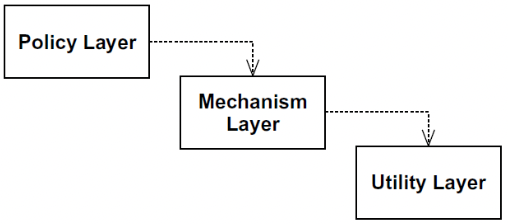
\includegraphics[width=2in]{DIPNaive}
				\scalebox{0.7}{\begin{tikzpicture}
						\node[type] (mechanism) {\Verb|Mechanism| \\ \Verb|Layer|};
						\node[type] (policy) [left=of mechanism, yshift=30pt]{\Verb|Policy| \\ \Verb|Layer|};
						\node[type] (utility) [right=of mechanism, yshift=-30pt] {\Verb|Utility| \\ \Verb|Layer|};

						\draw[dash pattern=on 2pt off 0.5pt, -{Straight Barb[width=2mm]}] (policy.east) -| (mechanism.north);
						\draw[dash pattern=on 2pt off 0.5pt, -{Straight Barb[width=2mm]}] (mechanism.east) -| (utility.north);
				\end{tikzpicture}}
			\end{center}
		\end{minipage}
		\begin{minipage}[t]{0.5\textwidth}
			\begin{center}
				\underline{\textbf{Inverted Layers}}\\
%				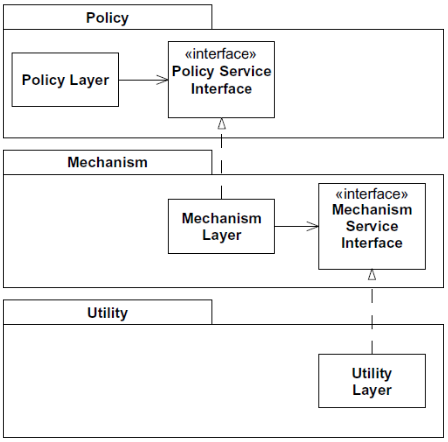
\includegraphics[width=2.5in]{DIPInverted}
				\scalebox{0.7}{
					\begin{tikzpicture}
						\node[type] (mechanism) {\Verb|Mechanism| \\ \Verb|Layer|};
						\node[type] (mechinterface) [right=of mechanism] {\textbf{$ \langle\langle $Interface$ \rangle\rangle $} \\ \Verb|Mechanism| \\ \Verb|Service| \\ \Verb|Interface|};
						\node[minimum width=3cm] [left=of mechanism] (ghostmech) {};

						\draw[-Straight Barb] (mechanism) -- (mechinterface);

						\node[type] (policyinterface) [above=1.9cm of mechanism] {\textbf{$ \langle\langle $Interface$ \rangle\rangle $} \\ \Verb|Policy Service| \\ \Verb|Interface|};
						\node[type] (policy) [left=of policyinterface] {\Verb|Policy Layer|};
						\node[minimum width=3cm] [right=of policyinterface] (ghostpolicy) {};

						\draw[-Straight Barb] (policy) -- (policyinterface);
						\draw[dash pattern=on 4pt off 2pt, -{Triangle[open, length=2.5mm, scale=1.3]}] (mechanism) -- (policyinterface);

						\node[type] (utilityinterface) [below=1.5cm of mechinterface] {\Verb|Utility| \\ \Verb|Layer|};
						\node[minimum width=3cm] (ghostutil1) [left=of utilityinterface] {};
						\node[minimum width=3cm] (ghostutil2) [left=of ghostutil1] {};
						\draw[dash pattern=on 4pt off 2pt, -{Triangle[open, length=2.5mm, scale=1.3]}] (utilityinterface) -- (mechinterface);

						\node[frame=black, fit=(mechanism)(mechinterface)(ghostmech)] (mech) {};
						\node[frame=black, fit=(policy)(policyinterface)(ghostpolicy)] (poli) {};
						\node[frame=black, fit=(utilityinterface)(ghostutil1)(ghostutil2)] (util) {};

						\node[draw, rectangle, above right, minimum width=2in] at (poli.north west) {Policy};
						\node[draw, rectangle, above right, minimum width=2in] at (mech.north west) {Mechanism};
						\node[draw, rectangle, above right, minimum width=2in] at (util.north west) {Utility};
					\end{tikzpicture}
				}
			\end{center}
		\end{minipage}
		\\[10pt]
		\begin{minipage}[t]{0.5\textwidth}
			\item Violating the DIP\\
%			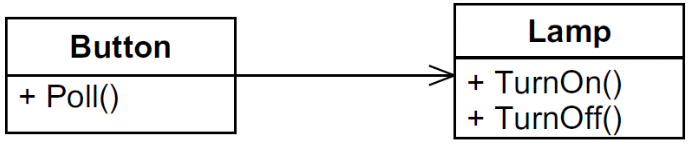
\includegraphics[width=2in]{DIPViolate}
			\scalebox{0.7}{
				\centering
				\begin{tikzpicture}
					\node[type] (lamp) {\Verb|Lamp|};
					\node[method] () [below=0pt of lamp] {+ turnOn()\\
						+ turnOff()};

					\node[type] (button) [left=of lamp] {\Verb|Button|};
					\node[method] () [below=0pt of button] {+ poll()};

					\draw[-Straight Barb] (button) -- (lamp);
				\end{tikzpicture}
			}
		\end{minipage}
		\begin{minipage}[t]{0.5\textwidth}
			\item Conforming to the DIP\\
%			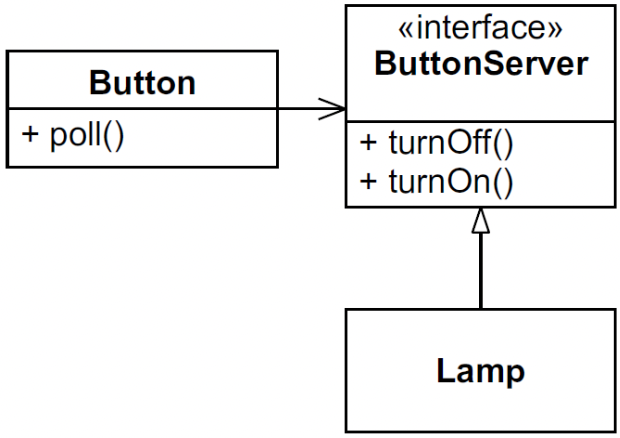
\includegraphics[width=2in]{DIPConform}
			\scalebox{0.7}{
				\begin{tikzpicture}
					\node[type] (buttonserver) {\Verb|<<Interface>>|\\
						\Verb|ButtonServer|};
					\node[method] (serverfn) [below=0pt of buttonserver] {+ turnOff()\\
						+ turnOn()};

					\node[type] (button) [left=of buttonserver] {\Verb|Button|};
					\node[method] () [below=0pt of button] {+ poll()};

					\node[type, minimum height=1.5cm] (lamp) [below=of serverfn] {\Verb|Lamp|};

					\draw[-Straight Barb] (button) -- (buttonserver);
					\draw[-{Triangle[open, length=2.5mm, scale=1.3]}] (lamp) -- (serverfn);
				\end{tikzpicture}
			}
		\end{minipage}
	\end{itemize}

	\item Design Smells
	\begin{itemize}
		\item Symptoms of poor design
		\item Often caused by the violation of one or more of the design principles
		\begin{itemize}
			\item For example, the smell of \textit{Rigidity} is often a result of insufficient attention to OCP.
		\end{itemize}
		\item These symptoms include:
		\begin{enumerate}
			\item Rigidity -- The design is hard to change.
			\item Fragility -- The design is easy to break.
			\item Immobility -- The design is hard to reuse.
			\item Viscosity -- It is hard to do the right thing.
			\item Needless Complexity -- Overdesign.
			\item Needless Repetition -- Mouse abuse.
			\item Opacity -- Disorganized expression.
		\end{enumerate}
	\end{itemize}
\end{itemize}

%\end{document}